%%%%%%%%%%%%%%%%%%%%%%%%%%%%%%%%%%%%%%%%%
% Full Length Professional CV
% LaTeX Template
% Version 2.0 (13/6/20)
%
% Original author:
% Sreedhar Unnikrishnakurup 
%
% Important note:
% This template requires the my_cv.cls file to be in the same directory as the .tex file. The my_cv.cls file provides the resume style used for structuring the document. THe publication.bib file is needed for adding the publication list
%
%%%%%%%%%%%%%%%%%%%%%%%%%%%%%%%%%%%%%%%%%

%----------------------------------------------------------------------------------------
%	PACKAGES AND OTHER DOCUMENT CONFIGURATIONS
%----------------------------------------------------------------------------------------

\documentclass{my_cv}% Use the custom my_cv.cls style
\begin{document}
\title{CV}
\author{Sreedhar Unnikrishnakurup}
\begin{minipage}{0.8\textwidth}
\begingroup
\let\center\flushleft
\let\endcenter\endflushleft
\maketitle
\endgroup
\end{minipage}
\begin{minipage}{0.1\textwidth}
\begin{tikzpicture}[remember picture,overlay]
\clip ($(current page text area.north east)!0.01!(current page text area.south east)!-7.4!(current page text area.north west)$)
  circle (2.1cm) node {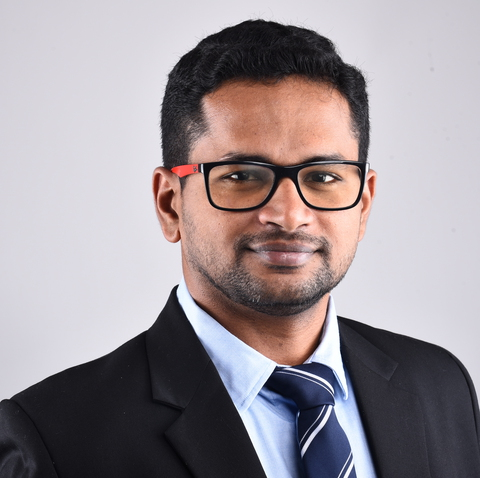
\includegraphics[width=2.3\linewidth]{mypic2}};
\end{tikzpicture}
%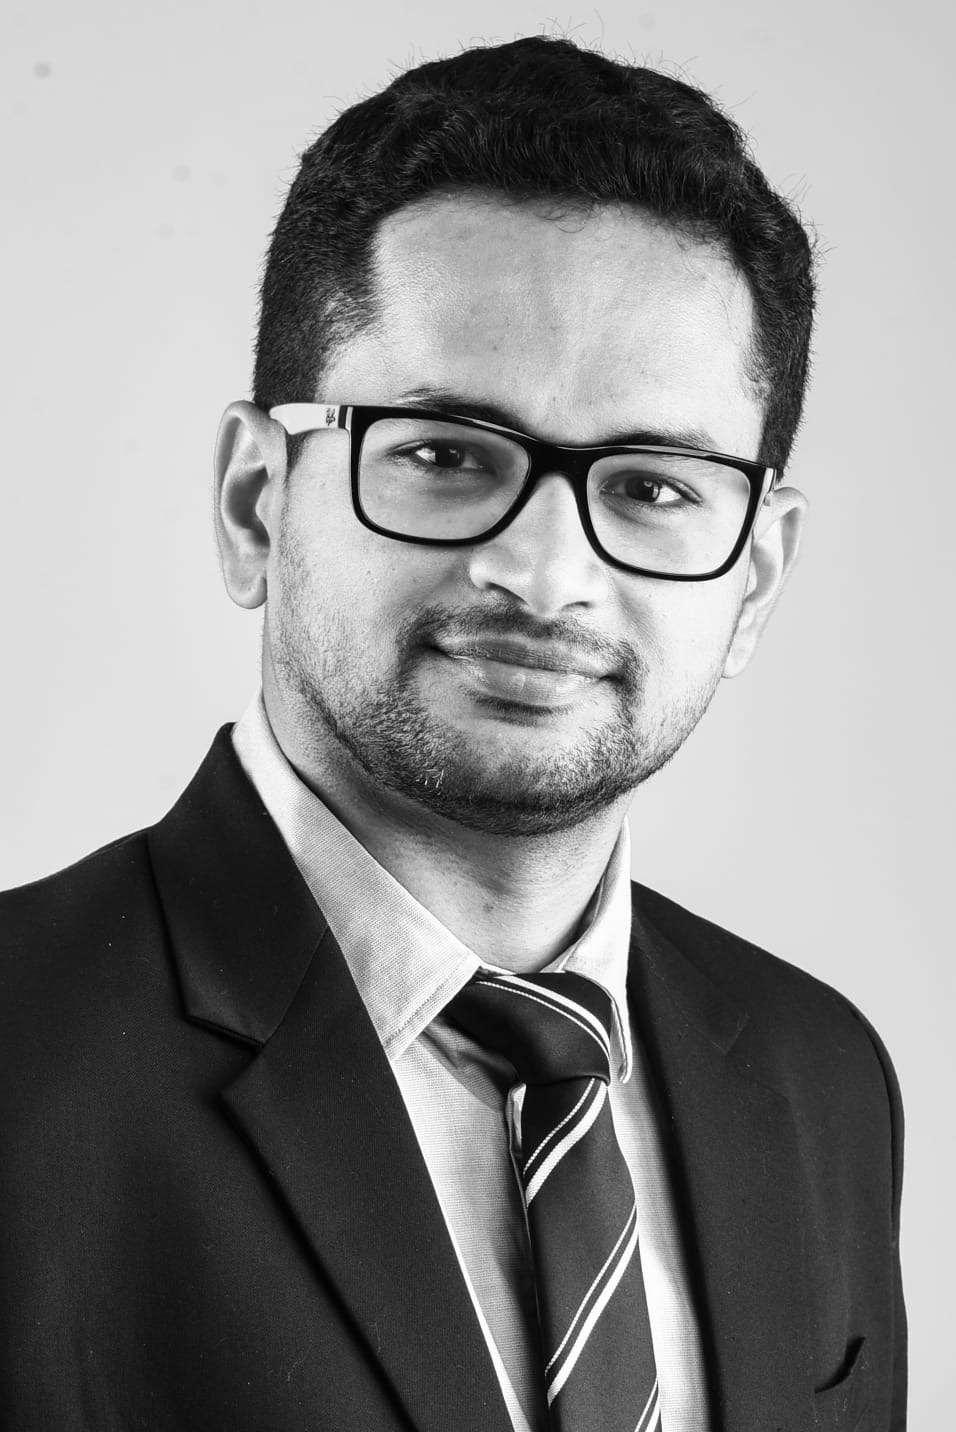
\includegraphics[width=8em]{mypic}
\end{minipage}
\vspace{1.5em}
%-------------------------------------------------------------
%	HIGHLIGHTS
%-------------------------------------------------------------
\section{Highlights}
\vspace{1.0em}
\begin{itemize}[leftmargin=0.15in]
\setlength\itemsep{-0.1em}
\color{mygray}
\item Postdoc experience in Online weld quality monitoring using Infrared Thermography (IRT), Pulsed IRT and THz-Time Domain spectroscopy (THz-TDS) for coating thickness inspection, composite inspection using pulsed IRT, lock-in IRT and Induction heating IRT, Laser IRT for crack inspection, Numerical study of heat transfer in Polycrystalline Microstructure, and X-ray radiography and Computed Tomography (CT) for weld inspection.
\item Ph.D. from University of Montpellier 2, France in Welding Engineering and Inverse analysis for multi-parameter optimization.
\item MS from Indian Institute of Technology (IIT) Madras in online monitoring of Weld quality using IRT and X-ray.
\item Age: 38 years
\end{itemize}
%-------------------------------------------------------------
%	WORK EXPERIENCE SECTION
%-------------------------------------------------------------
\section{Work Experience}
\vspace{1.0em}
\subsection{Scientist}
\subsubsection{\href{https://www.a-star.edu.sg/imre}{Institute of Material Research and Engineering (IMRE), A*STAR}}
\datedsubsection{Nov 2021-Ongoing}{Singapore}
%\paragraph{
\begin{itemize}[leftmargin=0.15in]
\setlength\itemsep{-0.1em}
\color{mygray}
\item Advanced Nondestructive Infrared Thermography applications
\item Composite inspection using induction heating IRT.
\item In-situ process monitoring of Additive Manufacturing using IRT
\end{itemize}%}
{\color{mygray1} \hdashrule[0.1ex]{18.8cm}{0.2mm}{1mm}}
\subsection{Postdoctoral Scientist}
\subsubsection{\href{https://www.cnde.in/}{Centre for Non-Destructive Evaluation (CNDE), IIT Madras}}
\datedsubsection{May 2018 - Sep 2021}{Chennai, India}
%\paragraph{
\begin{itemize}[leftmargin=0.15in]
\setlength\itemsep{-0.1em}
\color{mygray}
\item Application of Nondestructive IRT testing for thickness inspection of thermal barrier coatings and validation using THz-TDS and Eddy current testing.
\item Composite inspection using induction heating IRT.
\item Crack inspection in steel billets at elevated temperatures using Laser assisted IRT.
\item Development of artificial intelligence assisted advanced radiography imaging and automatic defect recognition of critical welds and high energy materials
\item Ray tracing algorithms for X-ray radiography simulations and CT reconstruction algorithms
\item Numerical investigation of anisotropic heat diffusion in polycrystalline and composite microstructures.
\end{itemize}%}
{\color{mygray1} \hdashrule[0.1ex]{18.8cm}{0.2mm}{1mm}}
%{\color{mygray} \rule{\linewidth}{0.5mm} }
\subsection{Cohort Member BA3}
\subsubsection{\href{https://www.joinef.com/}{Entrepreneur First}}
\datedsubsection{February 2020 - May 2020}{Bangalore, India}
\begin{itemize}[leftmargin=0.15in]
\setlength\itemsep{-0.1em}
\color{mygray}
\item Explored several interesting technological solutions, exploring the market, validating the technology, speaking to customers, and researching prototypes
\item The ideas that we worked on are detect and report quality-compromised and counterfeit drugs using a mobile cloud-based cost-effective hyper-spectral Imaging based AI device
\end{itemize}
{\color{mygray1} \hdashrule[0.1ex]{18.8cm}{0.2mm}{1mm}}
\subsection{Postdoctoral Research Scientist}
\subsubsection{\href{https://www.bam.de/Navigation/DE/Home/home.html}{NDT group 8.7, Federal Institute for Material Research and Testing (BAM)}}
\datedsubsection{January 2016 - June 2017}{Berlin, Germany}
\begin{itemize}[leftmargin=0.15in]
\setlength\itemsep{-0.1em}
\color{mygray}
\item Development of computational simulations to study the active thermographic testing for defect detection in composites
\item Pulsed, Lock-in, and Step heating IRT testing of fiber reinforced composites 
\item Optimize and validate active thermography as full-field, fast and non-contact NDE technique for quantitative testing of FRP structures
\end{itemize}
{\color{mygray1} \hdashrule[0.1ex]{18.8cm}{0.2mm}{1mm}}
\subsection{Visiting Research Scientist}
\subsubsection{\href{https://innowacje.zut.edu.pl/cooperationoffer/electromagnetic-methods-non-destructive-testing}{Electromagnetic NDT Research Group, West Pomeranian University (ZUT)}}
\datedsubsection{January 2015 - June 2015}{Szczecin, Poland}
\begin{itemize}[leftmargin=0.15in]
\setlength\itemsep{-0.1em}
\color{mygray}
\item Terahertz imaging and time domain analysis for material defect identification in Composite Wind turbine blades
\item Active Infrared Thermography for defect identification in composite materials - Numerical investigations of heat sink effects in the infrared inspecton of composites
\end{itemize}
{\color{mygray1} \hdashrule[0.1ex]{18.8cm}{0.2mm}{1mm}}
\subsection{Institute Postdoctoral Fellow}
\subsubsection{\href{https://www.cnde.in/}{Centre for Non-Destructive Evaluation (CNDE), IIT Madras}}
\datedsubsection{September 2014 - December 2015}{Chennai, India}
\begin{itemize}[leftmargin=0.15in]
\setlength\itemsep{-0.1em}
\color{mygray}
\item Numerical modelling of microstructural heat diffusion and ultrasonic wave propagation in Polycrystalline Materials
\item CMT welding process monitoring using IR thermography 
\item In-line laser thermography for Online Monitoring of steel billets to predict the surface cracks formed during the non-uniform cooling
\end{itemize}
{\color{mygray1} \hdashrule[0.1ex]{18.8cm}{0.2mm}{1mm}}
\subsection{Research Associate}
\subsubsection{\href{https://www.cnde.in/}{Centre for Non-Destructive Evaluation (CNDE), IIT Madras}}
\datedsubsection{April 2007 - December 2008}{Chennai, India}
\begin{itemize}[leftmargin=0.15in]
\setlength\itemsep{-0.1em}
\color{mygray}
\item Development of online weld quality monitoring for AA2219 liquid propellant tanks using Infrared Thermal Imaging and X-ray radiography
\item Developed a finite element model for the prediction of temperature profiles during welding
\end{itemize}
%-------------------------------------------------------------
%	EDUCATION SECTION
%-------------------------------------------------------------
\section{Education}
\vspace{2em}
\subsection{Ph.D. in Mechanical Engineering}
\subsubsection{\faInstitution \hspace{0.2em} \href{https://www.umontpellier.fr/en/}{University of Montpellier 2 (UM2)}}
\datedsubsection{2011 - 2014}{Montpellier, France}
\begin{itemize}[leftmargin=0.15in]
\setlength\itemsep{-0.1em}
\color{mygray}
\item Dissertation Topic: Weld pool shape identification using Multi-physics modelling and Experiments
\end{itemize}
{\color{mygray1} \hdashrule[0.1ex]{18.8cm}{0.2mm}{1mm}}
\subsection{M.S. in Mechanical Engineering}
\subsubsection{\faInstitution \hspace{0.2em} \href{https://www.iitm.ac.in/}{Indian Institute of Technology Madras}}
\datedsubsection{2008 - 2010}{Chennai, India}
\begin{itemize}[leftmargin=0.15in]
\setlength\itemsep{-0.1em}
\color{mygray}
\item Dissertation Topic: Online weld quality monitoring using Infrared Thermal Imaging
\item Cumulative Grade Point Average 8 out of 10
\end{itemize}
{\color{mygray1} \hdashrule[0.1ex]{18.8cm}{0.2mm}{1mm}}
\subsection{Bachelors in Mechanical Engineering}
\subsubsection{\faInstitution \hspace{0.2em} \href{https://www.ieindia.org/webui/iei-home.aspx}{Institution of Engineers India}}
\datedsubsection{2002 - 2006}{Kottayam, India}
\begin{itemize}[leftmargin=0.15in]
\setlength\itemsep{-0.1em}
\color{mygray}
\item Cumulative Grade Point Average 6.94 out of 10
\end{itemize}
%-------------------------------------------------------------
%	Publication
%-------------------------------------------------------------
\section{Publication}
\vspace{1em}
\nobibliography{publication}
%\bibliographystyle{unsrt}
\bibliographystyle{unsrtnat}
\begin{comment}
\subsection{\faBook \hspace{0.2em} \bfseries Dissertations}
\vspace{1em}
\begin{enumerate}
\setlength\itemsep{-0.1em}
\color{mygray}
 \item \bibentry{sreedhar2014} \cite{sreedhar2014}
 \item \bibentry{sreedhar2011} \cite{sreedhar2011}
\end{enumerate}
\end{comment}

\subsection{\faFileTextO \hspace{0.5em}\bfseries Journal Articles}
\vspace{1em}
\begin{enumerate}
\setlength\itemsep{-0.1em}
\color{mygray}
 \item \bibentry{Mercy2022} 
 \item \bibentry{Renil2022} 
 \item \bibentry{Dhruv2021} 
 \item \bibentry{Surendra2021} 
 \item \bibentry{Sreedhar2020} 
 \item \bibentry{Saini2020} 
 \item \bibentry{puthiyaveettil2020} 
 \item \bibentry{Nithin2019} 
\end{enumerate}
\begin{comment}
\subsection{\faFilePowerpointO \hspace{0.5em}\bfseries Conference Presentations}
\begin{enumerate}
\setlength\itemsep{-0.1em}
\color{mygray}
\item \bibentry{Sreeconf2022} \cite{Sreeconf2022}
\item \bibentry{Jyoticonf2020} \cite{Jyoticonf2020}
\item \bibentry{Surendraconf2020} \cite{Surendraconf2020}
\item \bibentry{Dhruv2019} \cite{Dhruv2019}
\item \bibentry{Sreedharconf2020} \cite{Sreedharconf2020}
\item \bibentry{Sruthiconf2018} \cite{Sruthiconf2018}
\item \bibentry{Nithinconf2018} \cite{Nithinconf2018}
\item \bibentry{Maierhoferconf2018} \cite{Maierhoferconf2018}
\item \bibentry{Krishnaconf2017} \cite{Krishnaconf2017}
\item \bibentry{Renilconf2016} \cite{Renilconf2016}
\item \bibentry{Nithinconf2016} \cite{Nithinconf2016}
\item \bibentry{Polomskiconf2016} \cite{Polomskiconf2016}
\item \bibentry{Kidanganconf2016} \cite{Kidanganconf2016}
\item \bibentry{Shivaprasadconf2015} \cite{Shivaprasadconf2015}
\item \bibentry{Sreedharconf2015} \cite{Sreedharconf2015}
\item \bibentry{Shivaprasadcomsolconf2015} \cite{Shivaprasadcomsolconf2015}
\item \bibentry{SreedharQIRTconf2015} \cite{SreedharQIRTconf2015}
\item \bibentry{SzymznikQIRTconf2015} \cite{SzymznikQIRTconf2015}
\item \bibentry{SreeQIRTconf2015} \cite{SreeQIRTconf2015}
\item \bibentry{SreeSGRconf2015} \cite{SreeSGRconf2015}
\item \bibentry{SreePolandconf2015} \cite{SreePolandconf2015}
\item \bibentry{Chadyconf2015} \cite{Chadyconf2015}
\item \bibentry{Barbaraconf2014} \cite{Barbaraconf2014}
\item \bibentry{Rouquetteconf2014} \cite{Rouquetteconf2014}
\item \bibentry{Sreedharconf2013} \cite{Sreedharconf2013}
\item \bibentry{Sreedharconf2012} \cite{Sreedharconf2012}
\item \bibentry{SreedharNconf2012} \cite{SreedharNconf2012}
\item \bibentry{Rouquetteconf2011} \cite{Rouquetteconf2011}
\item \bibentry{Sreedharconf2009} \cite{Sreedharconf2009}
\end{enumerate}
\end{comment}
%\item Complete list of conference publication URL: \href{https://bit.ly/30BlL05}{https://bit.ly/30BlL05}
%--------------------------------------------------------------
%	              RESEARCH INTEREST
%-------------------------------------------------------------
\section{Research Interest}
\vspace{1em}
\begin{normalsize}\color{mygray}With in the field of mechanical engineering and material Science, my research interests span the areas of Nondestructive Testing and Evaluation particularly in Infrared Thermal Imaging and X-ray radiography, Welding process, Online monitoring, Hyperspectral Imaging, Ray Tracing, Computational modeling, Microstructural based material modeling, Data driven scientific computing, Deep learning and Machine Learning.
\end{normalsize}

%--------------------------------------------------------------
%	                 Grants and Fellowships
%-------------------------------------------------------------
\section{Grants and Fellowships}
\vspace{1em}
\grantsubsection{Travel Grant to attend international scientific event from Council of Scientific \& industrial Research }{2019}
\grantsubsection{Visiting Researcher Fellowship under EU Project  Health Monitoring of Offshore Wind Farms (HEMOW)}{2015}
\grantsubsection{Institute Postdoctoral Research Grant from Indian Institute of Technology Madras}{2014-2015}
\grantsubsection{French research allowance from University of Montpellier for carrying out Ph.D.}{2011-2013}
\grantsubsection{Post-Graduate Fellowship: GATE from Govt. of India}{2008-2010}
%-------------------------------------------------------------
%	                 Certifications and Courses
%-------------------------------------------------------------
\begin{comment}
\section{Certifications and Courses}
\vspace{1em}
\begin{itemize}[leftmargin=0.15in]
\setlength\itemsep{-0.1em}
\color{mygray}
\item[\faCertificate] Deep Learning, a 5-course specialization by deeplearning.ai on Coursera. Specialization Certificate earned on September 23, 2018
\item[\faCertificate] Winter School on Artificial Intelligence, Infosys Center for Artificial Intelligence at IIIT Delhi 18-21st Jan, 2019
%\item[\faCertificate] Fundamentals of Data Science \& Deep learning course, PadhAI, One fourth labs, IIT Madras (Ongoing, July 2020)
\end{itemize}
\end{comment}
%-------------------------------------------------------------
\end{document}




\begin{comment}
\subsubsection{Dr. C. V. Krishnamurthy} 
\faAt \hspace{0.2em} \href{mailto:cvkm@iitm.ac.in}{cvkm@iitm.ac.in} \\
\faInstitution \hspace{0.2em} \href{http://iitm.irins.org/profile/61936}{Department of Physics, IIT Madras}
\subsubsection{}
\vspace{4.8em}
\end{comment}